\clearpage
\section*{\currfilename}

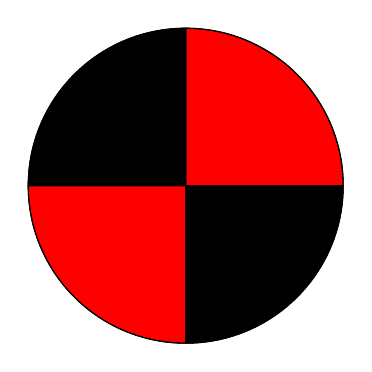
\begin{tikzpicture}[scale=1]
  \coordinate (BB) at (0,0);
  \coordinate (CC) at (2,0);
  \coordinate (DD) at (-2,0);
  \filldraw[black,fill=black] (BB)--(CC) arc (360:270:2) -- cycle;
  \filldraw[black,fill=red] (BB)--(CC) arc (0:90:2) -- cycle;
  \filldraw[black,fill=black] (BB)--(DD) arc (180:90:2) -- cycle;
  \filldraw[black,fill=red] (BB)--(DD) arc (180:270:2) -- cycle;
  \draw (BB) circle (2);
\end{tikzpicture}
